\documentclass[12pt]{article}
\usepackage[utf8]{inputenc}
\usepackage{amsmath}
\usepackage{graphicx}
\usepackage{float}
\usepackage[margin=1in]{geometry}
\usepackage{subcaption}
\usepackage{color}
\usepackage{lineno}
\usepackage{biblatex}
\addbibresource{Trial.bib}
\renewcommand\thelinenumber{\color{cyan}\arabic{linenumber}}
%%
\setlength{\parskip}{1em}
\setlength{\parindent}{0ex}
\renewcommand{\baselinestretch}{1.5}
\newcommand\dbyd[2]{\frac{\mathrm d{#1}}{\mathrm d{#2}}}
\newcommand\dsided[2]{{\mathrm d{#1}}/{\mathrm d{#2}}}
\newcommand{\R}{\mathcal{R}}
\title{Intentional infection as a method of\\population-level disease control}
\author{Roger Zhang}
\date{June 16th 2018}
\usepackage{color}
\newcommand{\david}[1]{\textcolor{blue}{$\langle${\slshape{\bfseries David:} #1 }$\rangle$}}
\newcommand{\roger}[1]{\textcolor{red}{$\langle${\slshape{\bfseries Roger:} #1 }$\rangle$}}
\usepackage[colorlinks=true,linkcolor=blue]{hyperref}
\newcommand{\pmV}{p_{V}}
\newcommand{\pmI}{p_{I}}


\begin{document}
\linenumbers
\maketitle
\begin{abstract}
In this paper, we study the possible advantages of intentional infection, as a method of population-level disease control. Intentional infection is a generalization of variolation, which was invented in 15th century, and widely used around the world in 17th and 18th century. People believed that variolation would result in a mild but protective infection, giving them a higher chance of survival than by being naturally infected. This paper aims to provide mathematical models describing the dynamics of infected classes, when intentional infection is introduced on a population level, and to perform predictions based on the models.
\end{abstract}
\clearpage
\tableofcontents
\clearpage
\section{Introduction}

Disease control has drawn people's attention since the early stage of human civilization. Other than curing diseases by medication, people have also discovered and attempted a vast range of method for disease prevention. Nowadays, people have vaccination as a primary method to prevent diseases \cite{bloom2006priorities}. However, before vaccination became a developed technology, people had limited power when encountering fatal diseases such as smallpox.

A practice called variolation was invented as an attempt to contain smallpox \cite{henderson1976eradication}. The earliest record of such method can be found in the 15th century, from an ancient Chinese documentation \cite{leung2011variolation}. It is a method used to immunize individuals against smallpox with materials taken from other smallpox patient, or from recently variolated individuals. People have found that, by variolation, a mild, but protective infection will likely occur \cite{leung2011variolation}. Instead of having a considerable chance of becoming gravely ill, a vast majority of variolated cases will survive after an infection. As a result, variolated individuals have a higher chance of survival.

More generally speaking, a similar method may be applied to other diseases for disease control. Fundamentally, since individuals are deliberately exposed to living virus, variolation is an example of intentional infection. Although an individual benefits from intentional infection when there is threat of being transmitted with fatal disease \cite{leung2011variolation}, people did not understand whether intentional infection can also bring positive effects when applied on a population level. 

Similar to vaccination, there are different strategies for variolation. One of strategies is to intentional infect newborn individuals \cite{dabrera2014case}. In fact, newborn infection does not mean instant infection when people are born, but rather an infection after their maternal immunity wanes \cite{elgert2009immunology}. Another strategy considered in this paper is to intentionally infect susceptible individuals in the population, at a fixed rate \cite{streefland1999patterns}. 

\section{Models: Intentional infect proportion of Newborn}
\subsection{Model: Modification to SIR model}
\subsubsection{System of differential equations}
We begin our analysis by modifying the SIR model. Our first strategy is to intentionally infect newborn individuals, with a certain proportion.  The following assumptions are made to simplify the model:
\begin{itemize}
\item No difference between intentionally infected and naturally infected individuals.
\item No disease induced mortality (disease induced mortality will be introduced in the later models).
\item Birth and natural death rate are the same (total population $N$ remains constant).
\item The latent period (time from infection to becoming infectious) is short enough to be ignored.
\item All susceptible individuals are equally likely to be infected, and all infected individuals are equally infectious.
\end{itemize}
Equipped with the assumptions above, we now setup our system of differential equations.

Just like in SIR model, $S$, $I$ and $R$ represent the proportion of susceptible, infected and recovered with respect to total population.
\begin{linenomath*}
\begin{equation}\label{1}
\begin{split}
\dbyd{S}{t}&=\mu(1-p)- \beta SI-\mu S \,,\\
\dbyd{I}{t}&=\beta SI+\mu p-\gamma I -\mu I\,,\\
\dbyd{R}{t}&=\gamma I-\mu R\,.
\end{split}
\end{equation}
\end{linenomath*}
Here, $\beta$ is the transmission rate, $\gamma$ is the recovery rate,
$\mu$ is the \emph{per capita} rate of birth and death, $p$ is the
proportion of newborns that are intentionally infected.

We non-dimensionalize \autoref{1} by scaling time, using
\begin{linenomath*}
\begin{equation}
\tau=(\gamma+\mu)t \,,
\end{equation}
\end{linenomath*}
so the time unit now is ``mean time infected".

The dimensionless system is:
\begin{subequations}\label{3}
\begin{linenomath*}
\begin{align}
\dbyd{S}{\tau}&=\epsilon(1-p)- \R_0  SI-\epsilon S \,,\\
\dbyd{I}{\tau}&=\R_0 SI+\epsilon p-I \,,
\end{align}
\end{linenomath*}
\end{subequations}
where $\epsilon=\frac{\mu}{\gamma+\mu}$, $\R_0=\frac{\beta}{\gamma+\mu}$.

We are not considering $\dbyd{R}{\tau}$ since it does not impact the dynamics of $S$ and $I$, and we do not need to track the proportion of recovered individuals in this model.
\subsubsection{Equilibria}
By setting \autoref{3} equal to 0, we solve for equilibria. The only equilibrium for this model is,
\begin{subequations}
\begin{linenomath*}
\begin{align}
\hat{S} &=\frac{1}{\R_0}-\frac{2p}{(\R_0 -1)+ \sqrt{(\R_0-1)^2+4\R_0 p}}\,, \label{Shat1}\\
\noalign{\vspace{10pt}}
\hat{I} &= \frac{\epsilon(\R_0 -1)+ \epsilon \sqrt{(\R_0-1)^2+4\R_0
    p}}{2\R_0}\,.\label{Ihat1}
\end{align}
\end{linenomath*}
\end{subequations}

Notice, \autoref{Ihat1} does not return 0 for any $p$ value between 0 and 1, meaning there is always infected individuals present in the population. Therefore, we can claim that this is not a disease free equilibrium. It follows that the equilibrium above is an endemic equilibrium (EE).

We would like to know if the EE is stable, therefore we need the Jacobian matrix of \autoref{3}. The Jacobian is, 
\begin{linenomath*}
\begin{equation}
\mathcal{J} =
\begin{bmatrix}
    \ -\R_0 I-\epsilon       & -\R_0 S \\
    \ \R_0 I       & \R_0 S-1 \\
\end{bmatrix} \,.
\end{equation}
\end{linenomath*}

Now for simplicity, let 
\begin{linenomath*}
\begin{equation}\label{E:}
K = (\R_0-1)+ \sqrt{(\R_0-1)^2+4\R_0 p} \,.
\end{equation}
\end{linenomath*}

For the purpose of our discussion, we are interested in disease that transmits fast enough to result in an epidemic. Therefore, the $\R_0$ value for the disease has to be greater than 1.

Notice, $K>0$ if $p\neq 0$.

Thus, the Jacobian evaluated at endemic equilibrium is,
\begin{linenomath*}
\begin{equation}
\mathcal{J}|_{EE} =
\begin{bmatrix}
    \ -\frac{\epsilon K}{2}-\epsilon       & -1+\frac{2p \R_0}{K} \\
    \ \frac{\epsilon K}{2}       & -\frac{2p \R_0}{K} \\
\end{bmatrix} \label{Jacobian1} \,,
\end{equation}
\end{linenomath*}

The eigenvalues of \autoref{Jacobian1} are,
\begin{linenomath*}
\begin{equation}
\lambda_{1,2} = \frac{-(\epsilon K^2+2\epsilon K +4p\mathcal{R}_0) \pm \sqrt{(\epsilon K^2+2\epsilon K +4p\mathcal{R}_0)^2-4(2\epsilon K^3+8\epsilon Kp\mathcal{R}_0)}}{4K}
\end{equation}
\end{linenomath*}

Since $(2\epsilon K^3+8\epsilon Kp\mathcal{R}_0)>0$, if the discriminant is positive, we have
\begin{linenomath*}
\begin{equation}
\sqrt{(\epsilon K^2+2\epsilon K +4p\mathcal{R}_0)^2-4(2\epsilon
  K^3+8\epsilon Kp\mathcal{R}_0)}
 \leq|\epsilon K^2+2\epsilon K +4p\mathcal{R}_0|  \,,
\end{equation}
\end{linenomath*}

thus, $\Re(\lambda_{1,2})<0$.

But if the discriminant is negative, we have
\begin{linenomath*}
\begin{equation}
\Re(\lambda_1)=\Re(\lambda_2)=-(\epsilon K^2+2\epsilon K +4p\mathcal{R}_0)<0  \,,
\end{equation}
\end{linenomath*}

As a result, we can conclude that EE is stable.

To fully investigate the dynamics of the system, we're also interested in whether the eigenvalues could be complex, which will lead to damped oscillation. 

Although it is difficult to determine the sign of the discriminant analytically, we can plot the value of the discriminant as a function of other parameter, i.e. $p$ or $\R_0$.

We begin our analysis with specific values of each parameter. Given the variolation history of smallpox, it is reasonable to adopt its parameter values as an example. The values are listed in \autoref{tab:params}.

\begin{table}[H]
\begin{center}
\caption{Model parameters and smallpox values.}
\label{tab:params}
\smallskip
\begin{tabular}{c|c|r}
{\bfseries Symbol} & {\bfseries Meaning} & {\bfseries Value} \\\hline
$\mu$ & Natural \emph{per capita} death rate & $\frac{1}{50*365}$ per day \\
$\gamma$ & Recovery rate & $\frac{1}{22}$ per day \\
$\R_0$ & Basic reproductive number & 4.5
\end{tabular}
\end{center}
\end{table}

\subsubsection{Region of $(\R_0,p)$ plane where there are damped
  oscillations (fixed $\epsilon$)}

$p$ is the proportion of intentional infection and $\R_0$ is the basic reproduction number.

\begin{figure}[h]
  \centering
  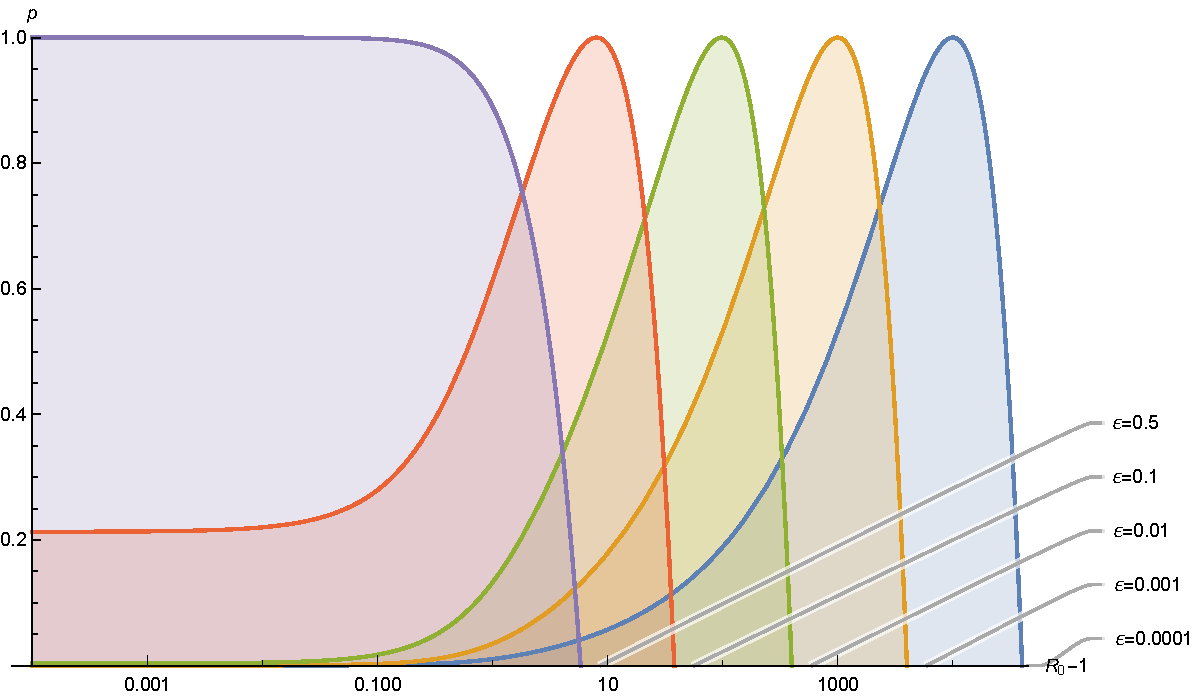
\includegraphics[width=0.9\textwidth]{Figures/Epsilons.pdf}
  \caption{The areas under each curve, shaded in different colors, represent the region of damped oscillations with respect to different $\epsilon$ values.}
\end{figure}

\subsubsection{Region of $(\R_0,\epsilon)$ plane where there are damped
  oscillations (fixed $p$)}

The plots below were made with different $p$ in increasing order, the shaded area between the blue curve and the orange curve represents the region where system has damped oscillation.

\begin{figure}[h]
\centering

\begin{subfigure}[t]{.4\textwidth}
\centering
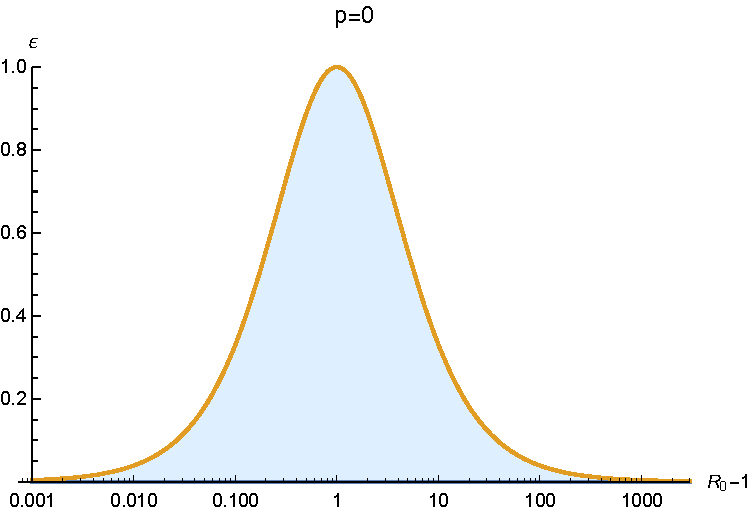
\includegraphics[width=\linewidth]{Figures/p_0.pdf}
        \caption{}\label{fig:fig_a}
\end{subfigure}
%
\begin{subfigure}[t]{.4\textwidth}
\centering
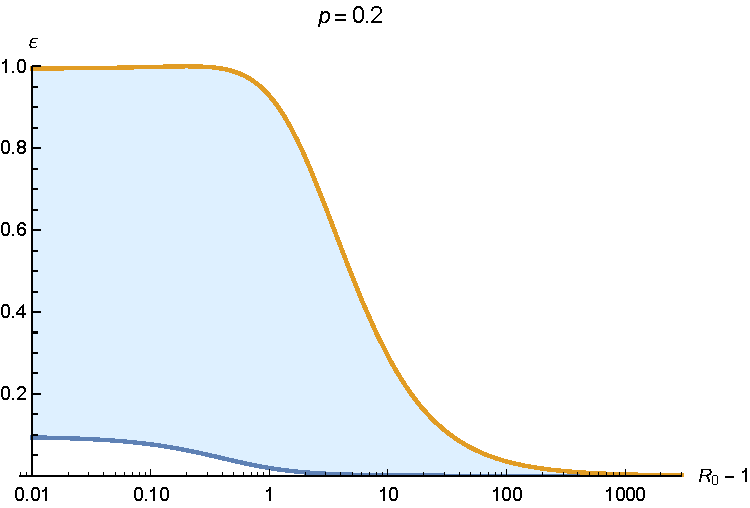
\includegraphics[width=\linewidth]{Figures/p_0_2.pdf}
\caption{}\label{fig:fig_b}
\end{subfigure}

\medskip

\begin{subfigure}[t]{.4\textwidth}
\centering
\vspace{0pt}% set the real top as the top
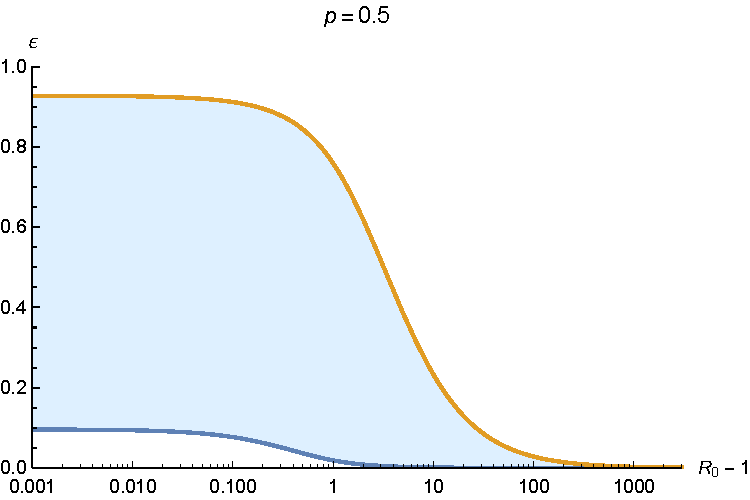
\includegraphics[width=\linewidth]{Figures/p_0_5.pdf}
\caption{}\label{fig:fig_c}
\end{subfigure}
%
\begin{subfigure}[t]{.4\textwidth}
\centering
\vspace{0pt}% set the real top as the top
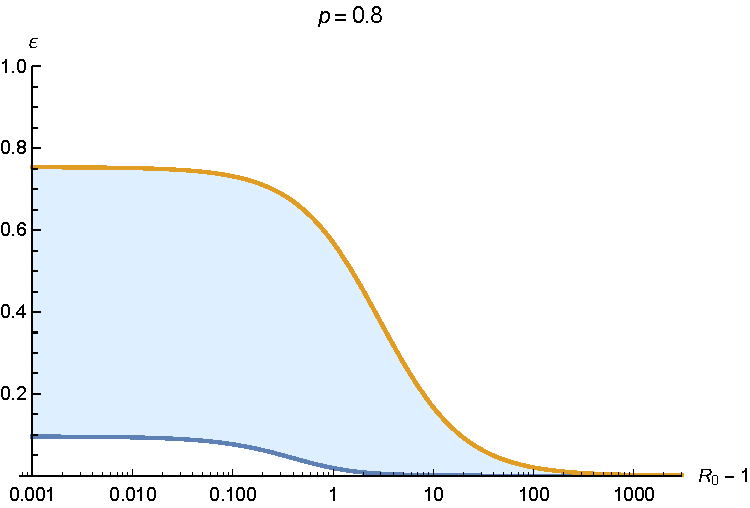
\includegraphics[width=\linewidth]{Figures/p_0_8.pdf}
\caption{}\label{fig:fig_d}
\end{subfigure}
%
\begin{minipage}[t]{0.9\textwidth}
\caption{Panel (a)-(d) illustrate $(\R_0,\epsilon)$ planes with different $p$ values. The shaded regions represent the range of conditions for damped oscillation to occur.\\ a) $p=0$, b) $p=0.2$,c) $p=0.5$, d) $p=0.8$}
\end{minipage}
\end{figure}

\clearpage

\subsubsection{Comments and discussion on this model}
This is the initial model of intentional infection on newborns, which we obtained by directly modifying standard SIR model. Notice, the main difference between intentional infection model and vaccination model is the direction of flow of individuals being treated with intentional infection or vaccination. Intentionally infected individuals are capable of transmitting the disease to susceptible individuals, whereas the vaccinated individuals will enter $R$(recovered) directly, therefore not being able to impact the dynamics of the system anymore. 

In our construction of the model, once an individual is intentionally infected, either directly or indirectly, this individual will not be naturally infected anymore. Therefore, we should divide the infected compartment into two separate infective classes, namely, intentionally infected and naturally infected.

In the past, for the case of smallpox, people believed that individuals that are variolated have a much better chance of survival, compared with naturally infected cases. Here we define ``advantageous'' as fewer total death. More specifically, we will be comparing total disease induced mortality. To achieve this, we need to involve a new parameter, namely, case fatality proportion.

\subsection{Model: Addition of disease induced mortality}\label{Newborn section}
\subsubsection{System of differential equations}
Disease induced mortality is created by deaths of infected population, with a ratio. This ratio is also known as case fatality proportion. 

Historic application of variolation have shown a lower case fatality proportion for those being variolated, compared to those being naturally infected. Thus, we need to assign different case fatality proportion to each class. This also requires us to divide $I$ from our previous model into two distinct infective classes, "Intentionally infected" ($V$) and "Naturally infected" ($I$). 

In this model, we still assume no latent period, and similar to the last assumption in our previous model, we assume that all infected individuals(including $V$ and $I$) are equally infectious.

After applying all assumptions, our model becomes,
\begin{linenomath*}
\begin{equation}\label{2}
\begin{split}
\dbyd{S}{t}&=\mu(1-p)- \beta S(V+I)-\mu S \,,\\
\dbyd{V}{t}&=\beta SV+\mu p-\gamma V -\mu V\,,\\
\dbyd{I}{t}&=\beta SI-\gamma I -\mu I\,,\\
\dbyd{M}{t}&=\pmV\gamma V+\pmI\gamma I\,,\\
\dbyd{R}{t}&=(1-\pmV)\gamma V+(1-\pmI)\gamma I-\mu R\,.
\end{split}
\end{equation}
\end{linenomath*}

In addition to the previous model, $\pmV$ and $\pmI$ represent the case fatality proportion for intentionally infected and naturally infected cases, respectively.

Again, we non-dimensionalize \autoref{2} by time, using
\begin{linenomath*}
\begin{equation}
\tau=(\gamma+\mu)t \,,
\end{equation}
\end{linenomath*}
which yields,
\begin{subequations}\label{eq:base_ODE}
\begin{linenomath*}
\begin{align}
\dbyd{S}{\tau}&=\epsilon(1-p)- \R_0 S(V+I)-\epsilon S\,, \label{eq:13a}\\
\dbyd{V}{\tau}&=\R_0 SV+\epsilon p-V\,, \label{eq:13b}\\
\dbyd{I}{\tau}&=\R_0 SI-I\,, \label{eq:13c}\\
\dbyd{M}{\tau}&=\pmV(1-\epsilon) V+\pmI(1-\epsilon) I\,, \label{eq:dMdtau}\\
\dbyd{R}{\tau}&=(1-\pmV)(1-\epsilon) V+(1-\pmI)(1-\epsilon) I-\epsilon R\,.
\end{align}
\end{linenomath*}
\end{subequations}
Notice here that $\R_0$, which is equal to $\frac{\beta}{\gamma+\mu}$, is again the basic reproduction number of the naturally infected cases. Since we assume that the transmission rate of naturally infected and intentionally infected cases are identical, $\R_0$ also plays a role as the basic reproduction number of intentionally infected cases. 

\subsubsection{Equilibria}

By setting \autoref{eq:13a}, \autoref{eq:13b} and \autoref{eq:13c} equal to 0, we solve for equilibria.

If $p=0$, meaning there is no intentional infection, our system reduces to the standard SIR model.

There are two equilibria for the standard SIR model, an Endemic equilibrium,
\begin{subequations}
\begin{linenomath*}
\begin{align}
\hat{S} &= \frac{1}{\R_0}\,,\\
\hat{V} &= 0\,,\\
\hat{I} &= \epsilon(1-\frac{1}{\R_0})\,.
\end{align}
\end{linenomath*}
\end{subequations}

And a disease free equilibrium(with both $\hat{V}$ and $\hat{I}$ are 0),
\begin{subequations}
\begin{linenomath*}
\begin{align}
\hat{S} &= 1\,,\\
\hat{V} &= 0\,,\\
\hat{I} &= 0\,.
\end{align}
\end{linenomath*}
\end{subequations}

However, if $p\neq 0$, there is only one equilibrium,
\begin{subequations}
\begin{linenomath*}
\begin{align}
\hat{S}&= \frac{1}{\R_0}-\frac{2p}{(\R_0 -1)+ \sqrt{(\R_0-1)^2+4\R_0
         p}}\,, \label{eq:3Shat}\\
\hat{V}&= \frac{\epsilon(\R_0 -1)+ \epsilon \sqrt{(\R_0-1)^2+4\R_0 p}}{2\R_0}\,, \label{eq:Vhat}\\
\hat{I}&=0\,. \label{eq:Ihat}
\end{align}
\end{linenomath*}
\end{subequations}

It is worthwhile mentioning that, since $\hat{V}\neq 0$, for any $p$ between 0 and 1, this equilibrium is not disease free. It follows that this equilibrium is the endemic equilibrium.

Stability analysis relies on Jacobian matrix, which is,
\begin{linenomath*}
\begin{equation}
\mathcal{J} =
\begin{bmatrix}
    \ -\R_0 (V+I)-\epsilon       & -\R_0 S     &-\R_0 S\\
    \ \R_0 V       & \R_0 S-1    &0\\
    \ \R_0 I       &0     &\R_0 S-1\\
\end{bmatrix}\,.
\end{equation}
\end{linenomath*}

Eigenvalues of Jacobian are given as follow. Here in our derivations, we are considering $S=\hat{S}$, $V=\hat{V}$.
\begin{subequations}
\begin{linenomath*}
\begin{align}
\lambda_1&=-1+\R_0 S \label{eq:3lambda1}\\
\lambda_2&=\frac{-1+\R_0 S-\epsilon-\R_0 V-\sqrt{(-1+\R_0 S-\epsilon-\R_0 V)^2-4(\R_0+\epsilon-\R_0 S\epsilon)}}{2} \label{eq:lambda2}\\
\lambda_3&=\frac{-1+\R_0 S-\epsilon-\R_0 V+\sqrt{(-1+\R_0 S-\epsilon-\R_0 V)^2-4(\R_0+\epsilon-\R_0 S\epsilon)}}{2}\label{eq:lambda3}
\end{align}
\end{linenomath*}
\end{subequations}
By using \autoref{eq:3Shat} and \autoref{eq:3lambda1}, we obtain
\begin{linenomath*}
\begin{equation}
-1+\R_0 S = - \frac{2p\R_0}{(\R_0 -1)+ \sqrt{(\R_0-1)^2+4\R_0 p}}<0
\end{equation}
\end{linenomath*}
Therefore,
\begin{linenomath*}
\begin{equation}
\Re(\lambda_1) =-1+\R_0 S<0\,.
\end{equation}
\end{linenomath*}
To determine the real part of $\lambda_2$ and $\lambda_3$, we need to determine the sign of the quantity under the square root in equation \autoref{eq:lambda2} and \autoref{eq:lambda3}. 

By using \autoref{eq:3Shat} again, we have
\begin{linenomath*}
\begin{equation}
\R_0 S\epsilon<\epsilon\,.
\end{equation}
\end{linenomath*}

Therefore,
\begin{linenomath*}
\begin{equation}
(\R_0+\epsilon-\R_0 S\epsilon)>\R_0 >0\,,
\end{equation}
\end{linenomath*}
which means, if the sign of the quantity under the square root is positive, we have
\begin{linenomath*}
\begin{equation}
\sqrt{(-1+\R_0 S-\epsilon-\R_0 V)^2-4(\R_0+\epsilon-\R_0 S\epsilon)}<|(-1+\R_0 S-\epsilon-\R_0 V)|
\end{equation}
\end{linenomath*}
Therefore, $\Re(\lambda_2)<\Re(\lambda_3)<0$.

Certainly, if the sign of the quantity under the square root is negative,
\begin{linenomath*}
\begin{equation}
\Re(\lambda_2)=\Re(\lambda_3)=-1+\R_0 S-\epsilon-\R_0 V<0
\end{equation}
\end{linenomath*}

We are able to conclude that EE is locally asymptotically stable.

We would also like to investigate the global stability of the EE. A Lyapunov function is usually required to conclude on the global stability of an equilibrium, but such function may not always be easily found. Therefore, instead of searching for a Lyapunov function, we will show global stability by simulating the system with random initial conditions. If the EE is globally asymptotically stable (GAS), the dynamics of the system should eventually converge to EE, regardless of the selection of the initial condition.

Here, we define a function that describes the distance between any point in the system to the EE. Knowing that EE is ($\hat{S}, \hat{V},\hat{I}$), the distance between any point ($S,V,I$) to the EE is given by:
\begin{equation}
d((S,V,I))=((\hat{S}-S)^2+(\hat{V}-V)^2+(\hat{I}-I)^2)^{\frac{1}{2}}
\end{equation}

If EE is GAS, the output of the distance function with any initial condition will eventually approach 0. If not, we will see the distance function unable to approach 0 for some initial conditions.

\begin{figure}[H]
  \centering
  \includegraphics[width=0.75\textwidth]{Figures/Model_1_2_distance_20.pdf}
  \caption{Distance between the dynamics of the system to EE, as a function of time. If EE is GAS, distance function should approach 0, indifferent of which initial condition was chosen. This figure shows the distance function of 50 random initial conditions. We have enough confidence to conclude that EE is GAS.}
\end{figure}

\subsubsection{Effect of intentional infection on total mortality}\label{section2.2.3}

In epidemic analysis, one way of measuring whether a certain intervention is more advantageous than another is to compare the total disease induced mortality. 

We first take a look at the mortality rate at EE, and insert $\hat{V}$ [\autoref{eq:Vhat}]
and $\hat{I}$ ($=0$) in \autoref{eq:dMdtau} to obtain
\begin{linenomath*}
\begin{equation}
\left. \dbyd{M}{\tau}\right|_{\rm EE}=\pmV(1-\epsilon)V=\frac{\pmV(1-\epsilon)\epsilon(\R_0 -1)+ \pmV(1-\epsilon)\epsilon \sqrt{(\R_0-1)^2+4\R_0 p}}{2\R_0}\,, \label{eq:dMdt}
\end{equation}
\end{linenomath*}

An important observation is that, at EE, mortality rate increases as $p$ increases. This shows in the long run, having a larger proportion of intentional infection is unwise as it leads to additional deaths.

In history, smallpox was present in the human population long before variolation was invented. When variolation was introduced, the population was already near equilibrium with no intentional infection ($p=0$). We are interested in the scenario where intentional infection is introduced after the population is in equilibrium without intentional infection.

One of the questions we want to answer is how long does our system take to reach the new EE. In fact, the system will reach the equilibrium only after infinite time.  Therefore, we need to define a threshold distance from the equilibrium that we consider to be ``at equilibrium''.
Since the new equilibrium has $\hat{I}=0$, we define reaching equilibrium by $I\leq 1\times 10^{-6}$ (one in a million).

If the case fatality proportion for intentionally infected cases is 1\%, we can hardly observe any difference when changing proportion of intentional infection. To help us observe the dynamics, we assume intentional infection has a 20\% case fatality proportion.

\autoref{figure:0.0001} shows that it takes shorter time to reach the new EE for a larger proportion of intentional infection.
\begin{figure}[h]
  \centering
  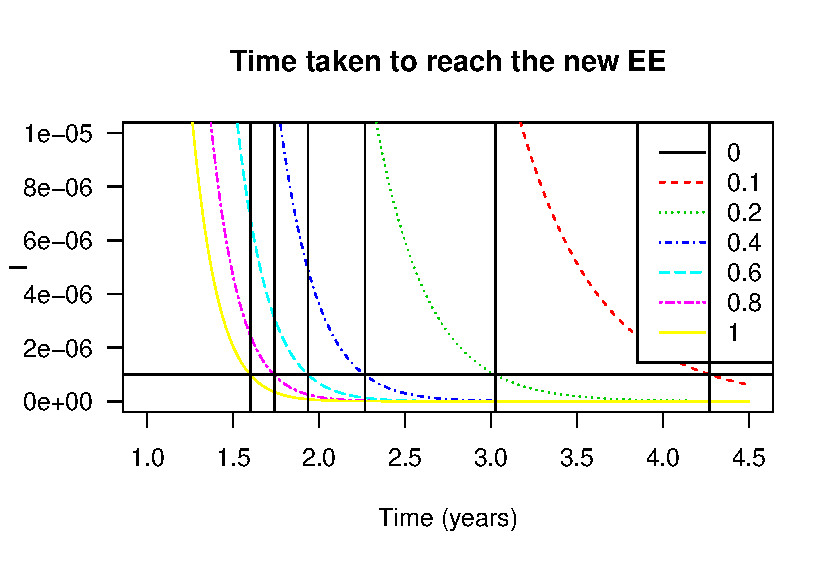
\includegraphics[width=0.9\textwidth]{Figures/I_less_than_0_000001.pdf}
  \caption{Determining time taken to reach equilibrium.  The horizontal line at $I=10^{-6}$ is the threshold we define to be ``at equilibrium''. This figure shows, with a larger proportion of intentional infection on newborn, the system reaches the equilibrium more quickly.}
\label{figure:0.0001}
\end{figure}

We are also interested in the time it takes for intentional infection to be more advantageous than non-intentional infection, by comparing total mortality.

From previous analysis, we have learned that $\dbyd{M}{\tau}$ decreases over time, and stabilizes at a constant rate when reaching the new EE. However, at the new EE, the magnitude of $\dbyd{M}{\tau}$ is larger when $p$ is larger.

\begin{figure}[H]
  \centering
  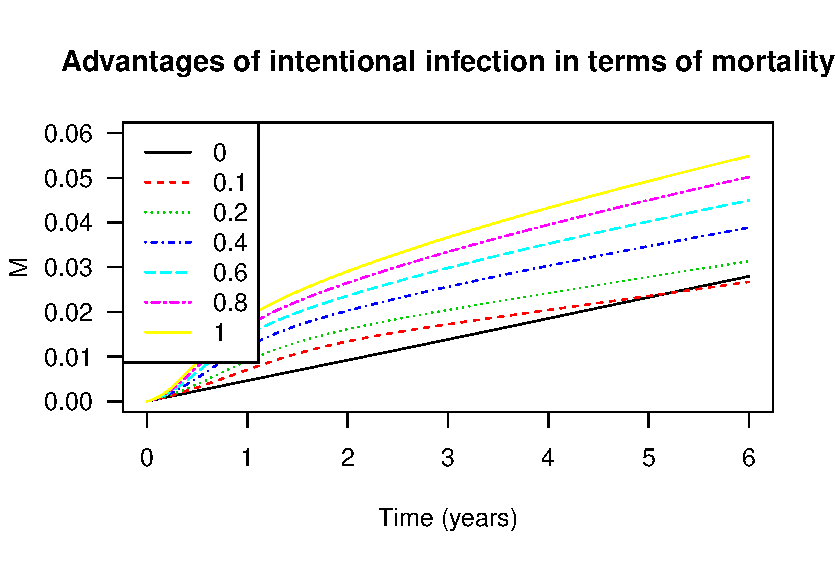
\includegraphics[width=0.9\textwidth]{Figures/dMdt.pdf}
  \caption{An illustration of intentional infection having advantages over non-intentional infection, with a case fatality proportion from intentional infection of $\pmV=0.2$.
Cumulative mortality ($M$) increases linearly with time without intentional infection ($p=0$, black line).
For any $p>0$, cumulative mortality is initially greater than for $p=0$, but eventually crosses the black line so is eventually lower (i.e., fewer deaths).}
\label{figure:advantage}
\end{figure}

\autoref{figure:advantage} shows, at earlier times, intentional infections have steeper slopes than the black line, which is non-intentional infection. The slopes for intentional infection decreases over time, and eventually intentional infection with any proportion will result in fewer total death than non-intentional infection.

\autoref{tab:times} summarize the time required to reach the new EE and the time required to have advantages over non-intentional infection.

\begin{table}[H]
\begin{center}
\caption{Time required to get close to the equilibrium ($\hat{I}<10^{-6}$) and time to gain advantages over non-intentional infection (i.e., lower cumulative mortality $M$).}
\label{tab:times}
\smallskip
\begin{tabular}{c|c|r}
{\bfseries $p$} & {\bfseries Time to EE} & {\bfseries Time to have advantages} \\\hline
0.1 & 4.27 yrs & 5.20 yrs \\
0.2 & 3.03 yrs & 8.81 yrs \\
0.4 & 2.27 yrs & 17.45 yrs \\
0.6 & 1.94 yrs & 28.37 yrs \\
0.8 & 1.74 yrs & 42.43 yrs \\
1.0 & 1.60 yrs & 61.46 yrs
\end{tabular}
\end{center}
\end{table}
Above table shows that as $p$ increases, the system reaches the new EE faster, but time required to gain advantages over the non-intentional infection case increases.

If we were to make the equivalent of \autoref{figure:advantage} with the CFP for intentional infection $\pmV=0.01$, then the time required to have advantages over non-intentional infection is minimal for any $p$ (the difference in time to advantage is less than a year regardless of the value of $p$).
\autoref{figure:advantage_by_p} shows the general relationship between time to advantage and $p$.

\begin{figure}[H]
  \centering
  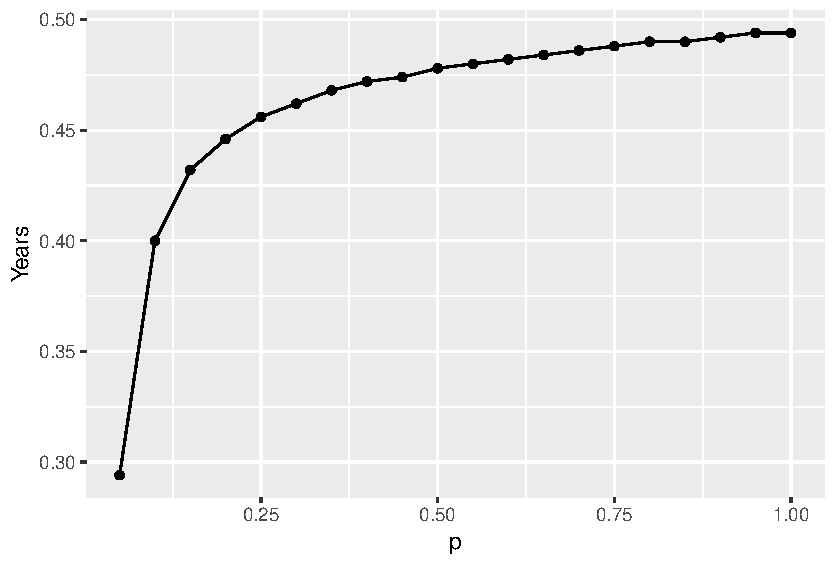
\includegraphics[width=0.9\textwidth]{Figures/Time_to_advantage_plot.pdf}
  \caption{Time to advantage as a function of $p$. The time required for intentional infection to be more advantageous than non-intentional infection increases as the proportion of intentional infection on newborn increases.}
\label{figure:advantage_by_p}
\end{figure}

\autoref{figure:advantage_by_p} shows that with a lower proportion of intentional infection $p$, we gain advantage faster. This conclusion is misleading, because it is suggesting that, with a minimal proportion of intentional infection, we can minimize the time it takes to gain advantage.
We found that, if $p$ is small, though it gains advantage faster, the number of deaths actually stays very close to non-intentional infection. In other words, although the advantage is obtained quickly, its magnitude is too small to be significant.  With this in mind, we will consider one intentional infection strategy ($p$ value) to be ``more advantageous'' than another if mortality with the strategic value of $p$ is at least 10\% lower than mortality with no intentional infection ($p=0$).

\begin{figure}[H]
  \caption{Time required for cumulative mortality of intentional infection becomes at least 10\% lower than of non-intentional infection. Under our new definition, with a larger proportion of intentional infection on newborn, intentional infections has fewer death than non-intentional infection in shorter time.}\label{advantage2}
  \centering
  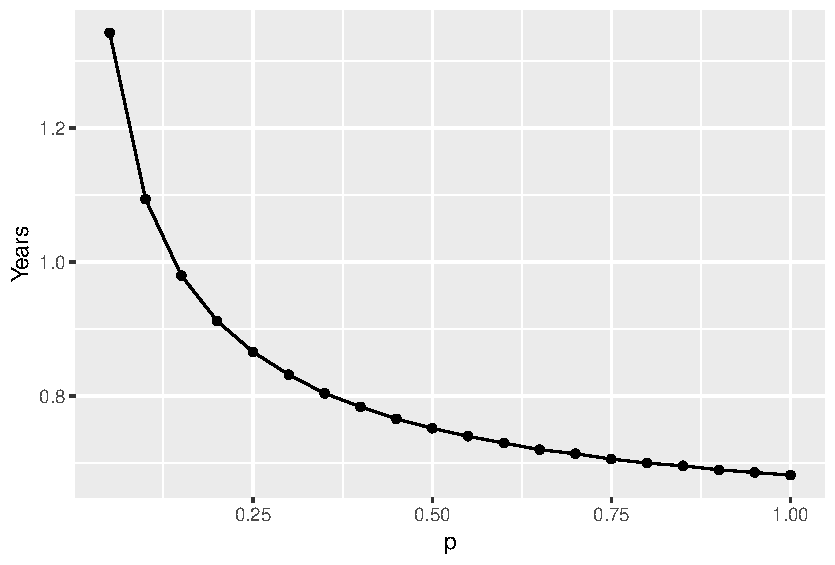
\includegraphics[width=1\textwidth]{Figures/New_time_to_advantage_plot.pdf}
\end{figure}
\autoref{advantage2} indicates that under our new definition of ``more advantageous'', the situation is reversed: a larger proportion of intentional infection yields an advantage more quickly.

\subsubsection{Comments and discussion on this model}

In this model, we have shown that intentional infection has an advantage over non-intentional infection in terms of total mortality. This suggests, in history, the introduction of intentional infection does have positive effects on disease control, intuitively by reducing the number of deaths. However, as we have discussed in the beginning of \autoref{section2.2.3}, a larger proportion of intentional infection on newborn will have a larger mortality rate once the equilibrium is reached. Though it can reduce total number deaths and become more advantageous than non-intentional infection faster, it is unwise to keep infecting such a large proportion of newborns simply because it will lead to more deaths. 

To summarize, if our strategy of intentional infection remains the same over time, in the long run, total mortality could be minimized with a minimal proportion of intentional infection. However, in a real life scenario, strategy does not need to be constant. It may be possible to intentionally infect at a relatively higher proportion initially, and decrease the proportion, or even stop intentional infection. With a combination of strategies like that, we could possibly minimize the total mortality, or even eradicate the disease.

Other than the possibilities of improving on the strategies of intentional infection, there could still be some development to the model itself to make it more suitable to a realistic scenario. For example, since Intentional infection has a lower death rate, we could assume a milder symptom for intentionally infected cases. As a result, because aggressive symptoms are typical routes of disease transmission, lack of such pathways will lead to a decrease in transmission rate. On the other hand, intentionally and naturally infected cases could have different recovery rates. Therefore, our next model could consider various possibilities of these parameters and draw conclusions to its behavior.

\subsubsection{Possibility of eradication}
If we define the disease as have been eradicated if the proportion of infected is less than one in a million, our model is able to predict possible eradication of the disease.

At EE, $I=0$. Although $I$ is going to approach 0 asymptotically, it will never completely cease to exist. However, because we know that there is a point in forward time where $I<1\times10^{-6}$, we can claim that naturally infected cases could be eradicated, this will be demonstrated in the next section.

The next question is whether it is possible for intentionally infected cases to burn out. After $I$ is wiped out, we can stop intentionally infecting any other newborns. From then on, if $S<\frac{1}{\R_0}$ for a long enough period of time, which means the effective $\R_0$ is less than 1, we could possibly observe $V<1\times10^{-6}$, which also represent the eradication of intentionally infected cases.

We use one example to illustrate the occurrence of such scenario. Assume we have $p=1$ until we reach EE, we could calculate $\hat{S}$ and $\hat{I}$. Now if we set the initial condition as $\hat{S}$ and $\hat{I}$ we just calculated and let $p=0$, we will obtain the following after simulation.
\begin{figure}[H]
  \centering
  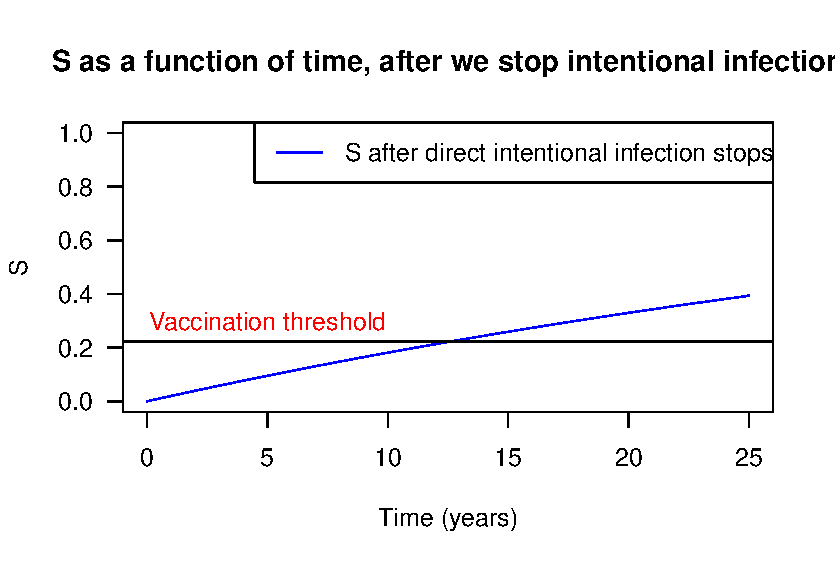
\includegraphics[width=1.1\textwidth]{Figures/Increase_of_S.pdf}
  \caption{The black line is the vaccination threshold for a disease with $\R_0=4.5$. The blue curve represent the dynamics of susceptible, after we stop intentional infection. This figure shows, for more than 10 years after we stop intentional infection, the amount of susceptible stays below the vaccination threshold.}
\label{figure:S_after_stop}
\end{figure}

\begin{figure}[H]
  \centering
  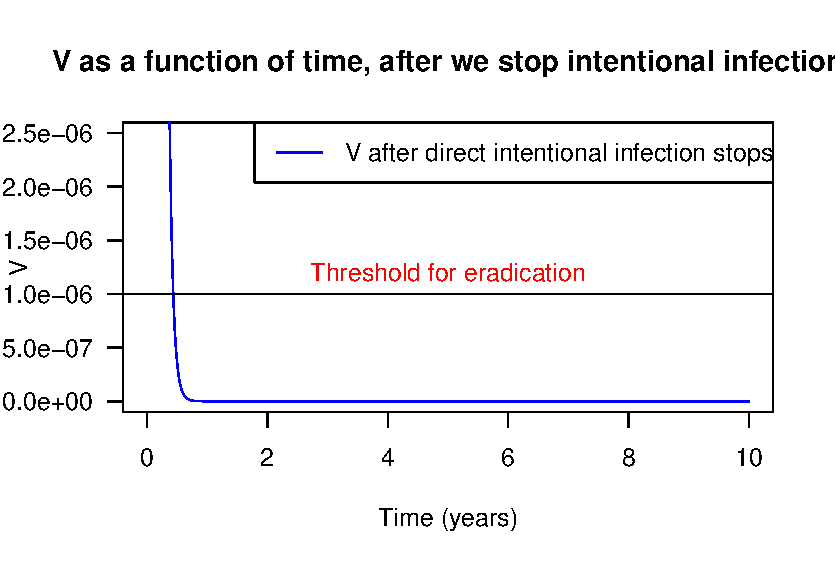
\includegraphics[width=1.1\textwidth]{Figures/V_after_stop.pdf}
  \caption{The black line is the pre-defined eradication threshold, $V=10^{-6}$. The blue curve represents the dynamics of V, after we stop intentional infection. This figure shows that it takes less than 1 year for $V$ to fall below the eradication threshold.}
\label{figure:V_after_stop}
\end{figure}

\autoref{figure:S_after_stop} and \autoref{figure:V_after_stop} have shown an example of pre-defined disease eradication. In our example, we assumed $p=1$, but other values of $p$ will still need to be investigated.

\subsection{Model: Different transmission rate and recovery rate}
\subsubsection{System of differential equations}
As mentioned above, we need to involve new parameters for different transmission and recovery rates. Here, let $\beta_V$ and $\beta_I$ represent the transmission rate of variolated cases and pathogen infected cases, respectively. $\gamma_V$ and $\gamma_I$ are the recovery rate of variolated cases and pathogen infected cases, respectively.

With the new parameters in hand, we now setup our system of differential equation,
\begin{linenomath*}
\begin{equation}\label{model:complex}
\begin{split}
\dbyd{S}{t}&=\mu(1-p)- \beta_V SV -\beta_I SI-\mu S \,,\\
\dbyd{V}{t}&=\beta_V SV+\mu p-\gamma_V V -\mu V\,,\\
\dbyd{I}{t}&=\beta_I SI-\gamma_I I -\mu I\,,\\
\dbyd{M}{t}&=\pmV\gamma_V V+\pmI\gamma_I I\,,\\
\dbyd{R}{t}&=(1-\pmV)\gamma_V V+(1-\pmI)\gamma_I I-\mu R\,.
\end{split}
\end{equation}
\end{linenomath*}

We non-dimensionalize \autoref{model:complex} by scaling time, by
\begin{linenomath*}
\begin{equation}
\tau=(\gamma_I+\mu)t \,.
\end{equation}
\end{linenomath*}

As the result, we obtain,
\begin{subequations}\label{eq:base_ODE}
\begin{linenomath*}
\begin{align}
\dbyd{S}{\tau}&=\epsilon(1-p)-\R_{0,V} SV-\R_{0,I} SI-\epsilon S\,, \label{eq:S_by_tau}\\
\dbyd{V}{\tau}&=\R_{0,V} SV+\epsilon p-\tilde{\gamma} V\,, \label{eq:V_by_tau}\\
\dbyd{I}{\tau}&=\R_{0,I} SI-I\,, \label{eq:I_by_tau}\\
\dbyd{M}{\tau}&=\pmV(\tilde{\gamma}-\epsilon) V+\pmI(1-\epsilon) I\,,\\
\dbyd{R}{\tau}&=(1-\pmV)(\tilde{\gamma}-\epsilon) V+(1-\pmI)(1-\epsilon) I-\epsilon R\,,
\end{align}
\end{linenomath*}
\end{subequations}

where $\R_{0,V}=\frac{\beta_V}{\gamma_I+\mu}$, $\R_{0,I}=\frac{\beta_I}{\gamma_I+\mu}$, $\tilde{\gamma}=\frac{\gamma_V+\mu}{\gamma_I+\mu}$, $\epsilon=\frac{\mu}{\gamma_I+\mu}$.

\subsubsection{Equilibria}

To solve for all equilibria, we set equations \autoref{eq:S_by_tau}, \autoref{eq:V_by_tau} and \autoref{eq:I_by_tau} equal to 0.

We acquired three solutions. However, given conditions that all $\hat{S}$, $\hat{V}$ and $\hat{I}$ have to be a non-negative number between 0 and 1, we can discard two of the solutions. The only solution left is, 
\begin{subequations}
\begin{linenomath*}
\begin{align}
\hat{S}&= \frac{\R_{0,V}+\tilde{\gamma}-\sqrt{\R_{0,V}^2-2\R_{0,V}\tilde{\gamma}+\tilde{\gamma}^2+4p\R_{0,V}\tilde{\gamma}}}{2\R_{0,V}}\,, \label{eq:Shat-1}\\
\hat{V}&= \frac{\epsilon-\frac{\tilde{\gamma}\epsilon}{\R_{0,V}}+\frac{\epsilon\sqrt{\R_{0,V}^2-2\R_{0,V}\tilde{\gamma}+\tilde{\gamma}^2+4p\R_{0,V}\tilde{\gamma}}}{\R_{0,V}}}{2\tilde{\gamma}}\,, \label{eq:Vhat-1}\\
\hat{I}&=0\,. \label{eq:Ihat-1}
\end{align}
\end{linenomath*}
\end{subequations}

Similar to our previous models, since infected population at equilibrium is non-zero, it is not a disease free equilibrium but rather an endemic equilibrium.

Stability analysis rely on Jacobian Matrix,
\begin{linenomath*}
\begin{equation}
\mathcal{J} =
\begin{bmatrix}
    \ -\R_{0,V}V-\R_{0,I}I-\epsilon       & -\R_{0,V}S     &-\R_{0,I}S\\
    \ \R_{0,V}V       & \R_{0,V}S-\gamma    &0\\
    \ \R_{0,I}I       &0     &\R_{0,I} S-1\\
\end{bmatrix}\,.
\end{equation}
\end{linenomath*}

Eigenvalues of Jacobian are given as follow,
\begin{subequations}
\begin{linenomath*}
\begin{align}
\lambda_1&=-1+\R_{0,I} S \label{eq:lambda1}\\
\lambda_2&=\frac{-\tilde{\gamma}+\R_{0,V}S-\epsilon-\R_{0,V}V-\sqrt{(-\tilde{\gamma}+\R_{0,V} S-\epsilon-\R_{0,V}V)^2-4(\R_{0,V}\tilde{\gamma}+\epsilon\tilde{\gamma}-\R_{0,V}S\epsilon)}}{2} \label{eq:lambda2-2}\\
\lambda_3&=\frac{-\tilde{\gamma}+\R_{0,V}S-\epsilon-\R_{0,V}V+\sqrt{(-\tilde{\gamma}+\R_{0,V} S-\epsilon-\R_{0,V}V)^2-4(\R_{0,V}\tilde{\gamma}+\epsilon\tilde{\gamma}-\R_{0,V}S\epsilon)}}{2}\label{eq:lambda3-3}
\end{align}
\end{linenomath*}
\end{subequations}

Looking at the real part of $\lambda_2$ and $\lambda_3$, first we look at the terms before square root. 

By using \autoref{eq:Shat-1}, we have
\begin{linenomath*}
\begin{equation}
-\tilde{\gamma}+\R_{0,V}S-\epsilon-\R_{0,V}V<0\,.
\end{equation}
\end{linenomath*}

Therefore,
\begin{linenomath*}
\begin{equation}
\Re(\lambda_2)<-\tilde{\gamma}+\R_{0,V}S-\epsilon-\R_{0,V}V<0\,.
\end{equation}
\end{linenomath*}

Next, notice
\begin{linenomath*}
\begin{equation}
\R_{0,V}\tilde{\gamma}+\epsilon\tilde{\gamma}-\R_{0,V}S\epsilon>0\,.
\end{equation}
\end{linenomath*}
It follows that
\begin{linenomath*}
\begin{equation}
\sqrt{(-\tilde{\gamma}+\R_{0,V} S-\epsilon-\R_{0,V}V)^2-4(\R_{0,V}\tilde{\gamma}+\epsilon\tilde{\gamma}-\R_{0,V}S\epsilon)}<|-\tilde{\gamma}+\R_{0,V} S-\epsilon-\R_{0,V}V|
\end{equation}
\end{linenomath*}
As the result, $\Re(\lambda_3)<0$.

Lastly, we look at $\lambda_1$. Here we noticed that $\Re(\lambda_1)$ is not necessarily negative as it depends on all other parameters. For the purpose of our interest, we would like to use specific value of smallpox to simulate the result.

We set $\R_{0,I}=4.5$. As $\R_{0,V}$ should be logically less than $\R_{0,I}$, we set $\R_{0,V}=2.5$, and plotted the ($\gamma,p$) plane.

\begin{figure}[H]
  \centering
  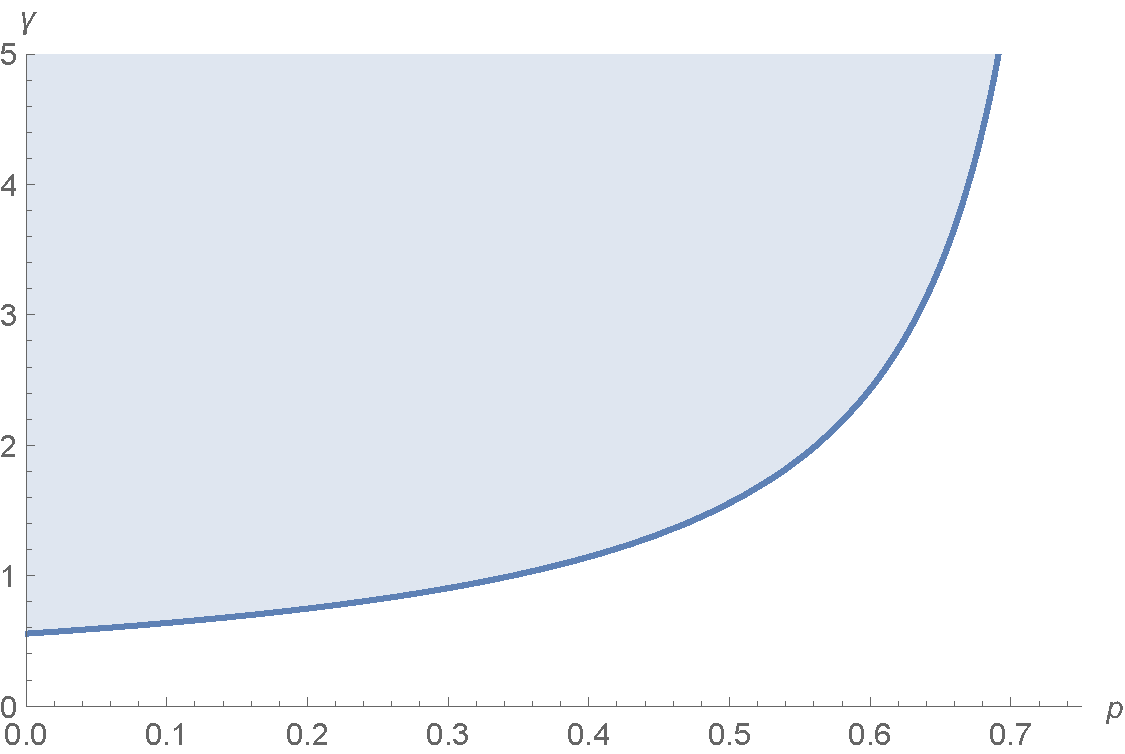
\includegraphics[width=1\textwidth]{Figures/Complex_model_eigenvalue_analysis.pdf}
  \caption{($\gamma,p$) plane when $\R_{0,V}=2.5, \R_{0,I}=4.5$. Shaded area is the region where $\Re(\lambda_1)<0$, meaning the system is locally asymptotically stable.}
\end{figure}

\subsubsection{Comments and discussion on this model}

Parameters of this model such as $\R_{0,V}$ and $\gamma_V$ can be immensely different depending on the design of the pathogen used for intentional infection. 

Previous studies have shown that, For a transmissible vaccine, in a similar model which does not consider natural birth and death, as well as no disease induced mortality. Even if $\R_{0,V}$ is less than 1, such as $\R_{0,V}=0.5$, a significant decrease in the final size of an epidemics is expected \cite{nuismer2018controlling}. In our model, birth and death rate are considered. Knowing that in our system, the disease can never be eradicated, there will always be newly infected cases. For that reason, we have an infinite population. Therefore, we cannot estimate final size for this model. But we are expecting that, the cumulative disease induced mortality will be reduced.

\section{Model: Intentionally infect susceptible with a certain rate}
\subsection{Model: Modification to SIR model}
\subsubsection{System of differential equations}
Our second strategy is to intentionally infect susceptible individuals with a certain rate. Again, we start our analysis by modifying the standard SIR model.

The following assumptions are made:
\begin{itemize}
\item No disease induced mortality.
\item Birth and natural death rate are the same, the total population remains constant.
\item Latent period is short enough to be ignored.
\item All susceptible individuals are equally likely to be infected, and all infected individuals are equally infectious.
\end{itemize}

\begin{linenomath*}
\begin{equation}\label{model:susceptible}
\begin{split}
\dbyd{S}{t}&=\mu- \beta SI-rS-\mu S\,, \\
\dbyd{I}{t}&=rS+\beta SI-\gamma I -\mu I\,,\\
\dbyd{R}{t}&=\gamma I-\mu R\,.
\end{split}
\end{equation}
\end{linenomath*}

Here, $\beta$ is transmission rate, $\gamma$ is recovery rate, $\mu$ is the \emph{per capita} rate of birth and death, $r$ is the rate of intensional infection on susceptible individuals. We will discuss the reasonable value of $r$ in later sections.

We convert our system into dimensionless form, by scaling time, by

\begin{linenomath*}
\begin{equation}
\tau=(\gamma+\mu)t\,.
\end{equation}
\end{linenomath*}

Therefore, the dimensionless system is:
\begin{linenomath*}
\begin{equation}
\begin{split}
\dbyd{S}{\tau}&=\epsilon- \R_0  SI-\eta S-\epsilon S\,, \\
\dbyd{I}{\tau}&=\eta S+\R_0 SI-I\,,\\
\dbyd{R}{\tau}&=(1-\epsilon)I-\epsilon R\,,
\end{split}
\end{equation}
\end{linenomath*}

where $\epsilon=\frac{\mu}{\gamma+\mu}$, $\R_0=\frac{\beta}{\gamma+\mu}$, $\eta=\frac{r}{\gamma+\mu}$.

\subsubsection{Equilibrium}
We obtain only one solution by solving the system:
\begin{subequations}
\begin{linenomath*}
\begin{align}
\hat{S} &= \frac{1}{\R_0}-\frac{2\eta}{\R_0(-(\eta+\epsilon-\epsilon\R_0)+\sqrt{(\eta+\epsilon-\epsilon\R_0)^2+4\R_0\epsilon \eta}+2\eta)}\\
\hat{I} &= \frac{-(\eta+\epsilon-\epsilon\R_0)+\sqrt{(\eta+\epsilon-\epsilon\R_0)^2+4\R_0\epsilon \eta}}{2\R_0}
\end{align}
\end{linenomath*}
\end{subequations}
Notice, for any non-zero $\eta$, $\hat{I}\neq 0$, it follows that this equilibrium is also an endemic equilibrium, since there is always proportion of population that are infected.

Stability analysis rely on Jacobian matrix, which is,
\begin{linenomath*}
\begin{equation}
\mathcal{J} =
\begin{bmatrix}
    \ -\R_0 I-\eta-\epsilon       & -\R_0 S \\
    \ \eta+\R_0 I       & \R_0 S-1 \\
\end{bmatrix}\,.
\end{equation}
\end{linenomath*}

For simplicity. Let 
\begin{linenomath*}
\begin{equation}
G=-(\eta+\epsilon-\epsilon\R_0)+\sqrt{(\eta+\epsilon-\epsilon\R_0)^2+4\R_0\epsilon \eta}.
\end{equation}
\end{linenomath*}
Notice, if $\epsilon,\eta\neq 0$, $G>0$. 

So Jacobian at EE becomes,
\begin{linenomath*}
\begin{equation}
\mathcal{J}|_{E.E.}=
\begin{bmatrix}
    \ \frac{G}{2}-\eta-\epsilon       & -1+\frac{2\eta}{G+2\eta} \\
    \ \eta+\frac{G}{2}       & -\frac{2\eta}{G+2\eta} \\
\end{bmatrix}\,.
\end{equation}
\end{linenomath*}

The eigenvalues of of Jacobian are:

\begin{linenomath*}
\begin{align}
\lambda_{1,2} &= \frac{-(G^2+4\eta G+2\epsilon G+4\eta^2+4\epsilon\eta+4\eta) }{4(G+2\eta)}\\
& \pm \frac{\sqrt{((G^2+4\eta G+2\epsilon G+4\eta^2+4\epsilon\eta+4\eta)^2-4(2G^3+12\eta G^2+24\eta^2 G+8\epsilon\eta G+16\eta^3+16\epsilon\eta^2)}}{4(G+2\eta)}
\end{align}
\end{linenomath*}

We know that $G>0$, and since the rate of intentional infection is non-zero, $\eta >0$

Since we are only interested in the case where the rate of intentional infection is non-zero, we assume that $\eta>0$. Together with the fact that $G>0$, the discriminant($\Delta$) satisfies the following inequality,
\begin{linenomath*}
\begin{equation}
\Delta<|(G^2+4\eta G+2\epsilon G+4\eta^2+4\epsilon\eta+4\eta)|
\end{equation}
\end{linenomath*}

Therefore, we can conclude that Re($\lambda$)$<0$, which means, EE is stable.

For global stability analysis, we applied the same method as in previous section, which is by using distance function.

The identical distance function was used to run the simulation, and the result is obtain in the following plot:

\begin{figure}[H]
  \centering
  \includegraphics[width=0.75\textwidth]{Figures/Model_2_2_distance_20.pdf}
  \caption{Distance between the dynamics of the system to the EE, as a function of time. If EE is GAS, distance function should approach 0, no matter which initial condition is chosen. This figure shows the distance function of 50 random initial conditions. We have enough confidence to conclude that EE is GAS.}
\end{figure}

To fully understand the dynamics of the system, we want to know whether or not there is a damped oscillation. This is done by determining the sign of the discriminant.

We will start our analysis with specific values of each parameter. Again, we will use parameters of smallpox. The values are listed in \autoref{tab:params}.
\subsubsection{Region of ($\R_0$,$\eta$) plane where there are damped oscillations (fixed $\epsilon$)}

$\eta$ is the rate of intentional infection, $\R_0$ is the basic reproduction number.

\begin{figure}[h]
\centering

\begin{subfigure}[t]{.4\textwidth}
\centering
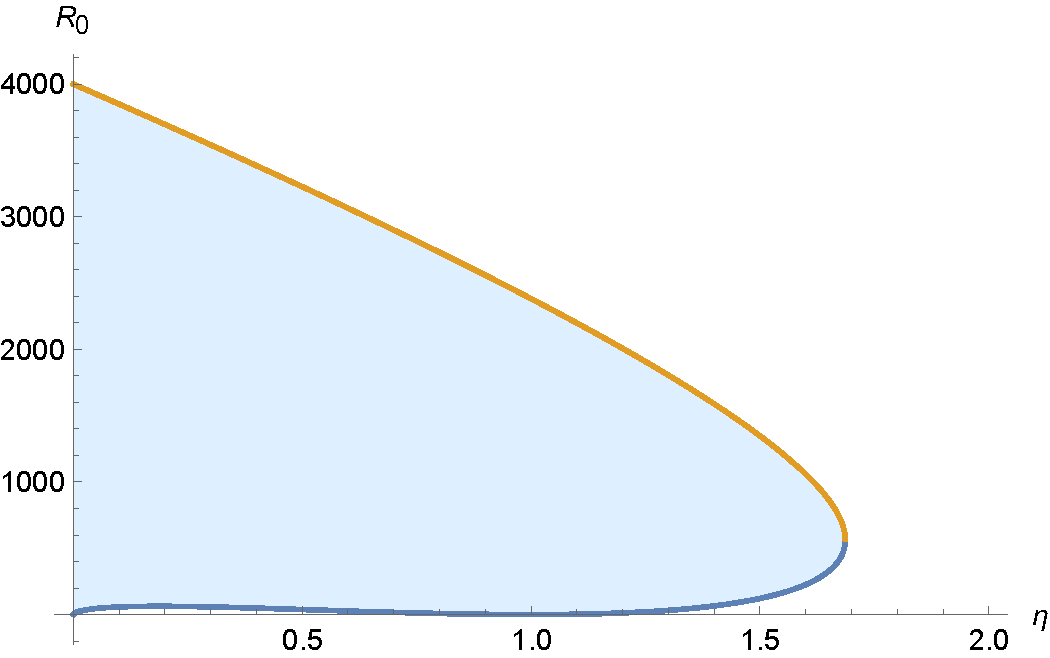
\includegraphics[width=\linewidth]{Figures/sus0_001.pdf}
        \caption{}\label{fig:fig_aa}
\end{subfigure}
%
\begin{subfigure}[t]{.4\textwidth}
\centering
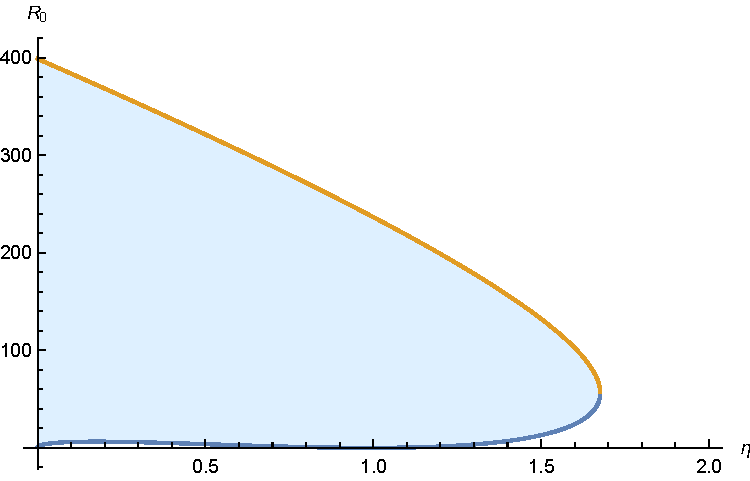
\includegraphics[width=\linewidth]{Figures/sus0_01.pdf}
\caption{}\label{fig:fig_bb}
\end{subfigure}

\medskip

\begin{subfigure}[t]{.4\textwidth}
\centering
\vspace{0pt}% set the real top as the top
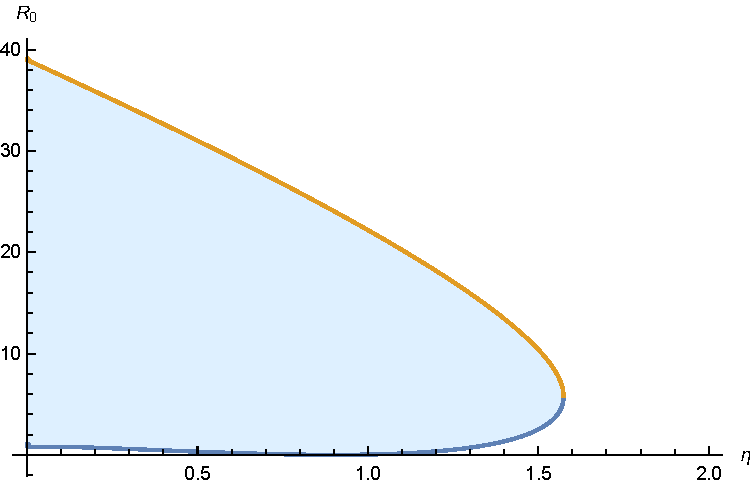
\includegraphics[width=\linewidth]{Figures/sus0_1.pdf}
\caption{}\label{fig:fig_cc}
\end{subfigure}
%
\begin{subfigure}[t]{.4\textwidth}
\centering
\vspace{0pt}% set the real top as the top
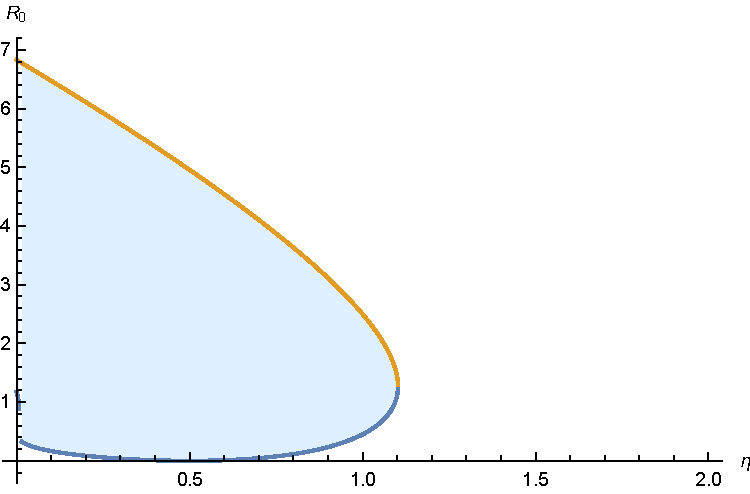
\includegraphics[width=\linewidth]{Figures/sus0_5.pdf}
\caption{}\label{fig:fig_dd}
\end{subfigure}
%
\begin{minipage}[t]{0.9\textwidth}
\caption{Panel (a)-(d) show ($\R_0,\eta$) plane for different $\epsilon$ values. The shaded region represent the range of conditions where the system has damped oscillations.\\
a) $\epsilon=0.001$, b) $\epsilon=0.01$, c) $\epsilon=0.1$, d) $\epsilon=0.5$}
\end{minipage}
\end{figure}

\subsubsection{Comments and discussion on this model}
Similar to our newborn infection model, the model obtained by modifying the standard SIR model is rather simple. We will still need to divide the infected compartment into intentionally and naturally infected classes.

Furthermore, to help us conclude whether or not there is any positive effect by intentionally infecting, we will need to involve disease induced mortality. This may also help us compare two different strategies of intentional infection.

\subsection{Model: Addition of disease induced mortality}

\subsubsection{System of differential equations}

The addition of disease induced mortality will require the involvement of case fatality proportion, again. 

Here, we are doing exactly the same adjustment as we did in \autoref{Newborn section}.
Our new system is,

\begin{subequations}\label{11}
\begin{linenomath*}
\begin{align}
\dbyd{S}{t}&=\mu- \beta S(V+I)-rS-\mu S \,,\\
\dbyd{V}{t}&=\beta SV+rS-\gamma V -\mu V\,,\\
\dbyd{I}{t}&=\beta SI-\gamma I -\mu I\,,\\
\dbyd{M}{t}&=\pmV\gamma V+\pmI\gamma I\,,\\
\dbyd{R}{t}&=(1-\pmV)\gamma V+(1-\pmI)\gamma I-\mu R\,,
\end{align}
\end{linenomath*}
\end{subequations}
where $\beta$ is transmission rate, $\gamma$ is recovery rate, $\mu$ is the \emph{per capita} rate of birth and death, $r$ is the rate of intensional infection on susceptible individuals.

We non-dimensionalize \autoref{11} by scaling time, by
\begin{linenomath*}
\begin{equation}
\tau=(\gamma+\mu)t \,,
\end{equation}
\end{linenomath*}

As the result, we obtain,

\begin{subequations}\label{eq:base}
\begin{linenomath*}
\begin{align}
\dbyd{S}{\tau}&=\epsilon-\eta S-\R_0 S(V+I)-\epsilon S\,, \label{3a}\\
\dbyd{V}{\tau}&=\R_0 SV+\eta S-V\,, \label{3b}\\
\dbyd{I}{\tau}&=\R_0 SI-I\,, \label{3c}\\
\dbyd{M}{\tau}&=\pmV(1-\epsilon) V+\pmI(1-\epsilon) I\,,\\
\dbyd{R}{\tau}&=(1-\pmV)(1-\epsilon) V+(1-\pmI)(1-\epsilon) I-\epsilon R\,,
\end{align}
\end{linenomath*}
\end{subequations}

Where $\epsilon=\frac{\mu}{\gamma+\mu}$, $\R_0=\frac{\beta}{\gamma+\mu}$, $\eta=\frac{r}{\gamma+\mu}$

\subsubsection{Equilibria}
If $\eta=0$, the system will again be simplified to the standard SIR model, the equilibrium of that has been shown before. Here, we are only interested in the case where $\eta\neq0$.

The only solution we obtain by solving the system is:

\begin{subequations}\label{eq:EE}
\begin{linenomath*}
\begin{align}
\hat{S} &= \frac{1}{\R_0}-\frac{2\eta}{\R_0(-(\eta+\epsilon-\epsilon\R_0)+\sqrt{(\eta+\epsilon-\epsilon\R_0)^2+4\R_0\epsilon \eta}+2\eta)}\,, \label{eq:Shat-11}\\
\hat{V} &= \frac{-(\eta+\epsilon-\epsilon\R_0)+\sqrt{(\eta+\epsilon-\epsilon\R_0)^2+4\R_0\epsilon \eta}}{2\R_0}\,, \label{eq:Vhat-11}\\
\hat{I} &= 0\,,
\end{align}
\end{linenomath*}
\end{subequations}

Notice, $\hat{V}$ is non-zero, therefore this equilibrium is not a disease free equilibrium. It follows that it is the endemic equilibrium.

\subsubsection{Stability of Endemic Equilibrium}

The Jacobian matrix of this system is,
\begin{linenomath*}
\begin{equation}
\mathcal{J} =
\begin{bmatrix}
    \ -\eta-\R_0 (V+I)-\epsilon       & -\R_0 S     &-\R_0 S\\
    \ \R_0 V+\eta       & \R_0 S-1    &0\\
    \ \R_0 I       &0     &\R_0 S-1\\
\end{bmatrix}\,.
\end{equation}
\end{linenomath*}

Eigenvalues of Jacobian are ,
\begin{subequations}
\begin{linenomath*}
\begin{align}
\lambda_1&=-1+\R_0 S \label{eq:lambda1}\\
\lambda_2&=\frac{-1+\R_0 S-\eta-\epsilon-\R_0 V+\sqrt{(-1+\R_0 S-\eta-\epsilon-\R_0 V)^2-4(\eta+\R_0 V+\epsilon-\R_0 S\epsilon)}}{2}\\
\lambda_3&=\frac{-1+\R_0 S-\eta-\epsilon-\R_0 V-\sqrt{(-1+\R_0 S-\eta-\epsilon-\R_0 V)^2-4(\eta+\R_0 V+\epsilon-\R_0 S\epsilon)}}{2}
\end{align}
\end{linenomath*}
\end{subequations}

By using \autoref{eq:Shat-11} and \autoref{eq:lambda1}, we get
\begin{linenomath*}
\begin{equation}
\Re(\lambda_1)=-1+\R_0 S=-\frac{2\eta}{(-(\eta+\epsilon-\epsilon\R_0)+\sqrt{(\eta+\epsilon-\epsilon\R_0)^2+4\R_0\epsilon \eta}+2\eta)}<0
\end{equation}
\end{linenomath*}

To decide the real parts of $\lambda_2$ and $\lambda_3$, we need to determine the sign of the quantity under the square root.

By using \autoref{eq:Shat-11} again, we have
\begin{linenomath*}
\begin{equation}
\R_0 S\epsilon<\epsilon\,,
\end{equation}
\end{linenomath*}

Therefore
\begin{linenomath*}
\begin{equation}
(\eta+\R_0 V+\epsilon-\R_0 S\epsilon)>0\,,
\end{equation}
\end{linenomath*}

It follows that
\begin{linenomath*}
\begin{equation}
\sqrt{(-1+\R_0 S-\eta-\epsilon-\R_0 V)^2-4(\eta+\R_0 V+\epsilon-\R_0 S\epsilon)}<|(-1+\R_0 S-\eta-\epsilon-\R_0 V)|\,.
\end{equation}
\end{linenomath*}

It follows that we have two cases, if the quantity under square root is negative, then
\begin{linenomath*}
\begin{equation}
\Re(\lambda_2)=\Re(\lambda_3)=-1+\R_0 S-\eta-\epsilon-\R_0 V<0\,,
\end{equation}
\end{linenomath*}

Otherwise, we have
\begin{linenomath*}
\begin{equation}
\Re(\lambda_3)<\Re(\lambda_2)<0
\end{equation}
\end{linenomath*}

Thus, for any $\eta>0$, we can conclude that the EE is locally asymptotically stable regardless of the values of other parameters.

\subsubsection{The effect of intentional infection on mortality}
We will again start by looking at the mortality rate at EE.

By inserting $\hat{V}$[\autoref{eq:Vhat-11}] and $\hat{I}$ ($=0$) into \autoref{eq:base}, we obtain the mortality rate at EE,
\begin{linenomath*}
\begin{equation}
\dbyd{M}{\tau}=\pmV(1-\epsilon)V=\frac{\pmV(1-\epsilon)\epsilon(\R_0 -1)+ \pmV(1-\epsilon)\epsilon \sqrt{(\R_0-1)^2+4\R_0 p}}{2\R_0}\,, \label{eq:dMdt}
\end{equation}
\end{linenomath*}
as shown the following graph,
\begin{figure}[H]
  \centering
  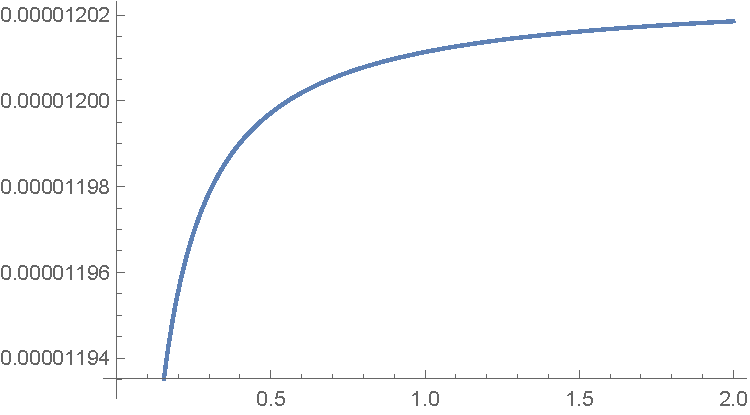
\includegraphics[width=1\textwidth]{Figures/M_at_EE.pdf}
  \caption{$\dbyd{M}{\tau}$ at EE as a function of $\eta$. $\dbyd{M}{\tau}$ increases as the rate of intentional infection on susceptible increase. The magnitude of $\dbyd{M}{\tau}$ eventually reaches an asymptote at $\dbyd{M}{\tau}=0.00001202$.}
\end{figure}

It is worthwhile noticing that, as we increase the rate of intentional infection, the mortality rate eventually reaches an asymptote at around $1.2\times10^{-5}$, which is very close to the mortality rate when we intentionally infect newborn individuals with a highest proportion ($p=1$). This suggests, in the long run, a high proportion of newborn infection would have similar results as intentionally infect susceptible at a high rate. A logical explanation to that is, when $p=1$ for newborn infection model or when $r$ is very high for susceptible model, at EE, there is almost nobody that is still susceptible ($\hat{S}=0$ or $\hat{S}\approx0$). The only individuals entering the system are the newborns, but newborn model will intentionally infect 100\% of them before they become susceptible. Similarly, susceptible model will intentionally infect almost all of them immediately after they become susceptible. As a result, the increasing rates of $V$ (intentionally infected) are essentially the same for both approaches. Therefore, due to the fact that $\dbyd{M}{\tau}$ is directly proportional to $\hat{V}$, the magnitude of $\dbyd{M}{\tau}$ are similar.


As we did in the newborn model, we also want to know the time it takes for susceptible intentional infection to reach the new equilibrium, as well as the time it takes to be advantageous over non-intentional infection.

\begin{figure}[H]
  \centering
  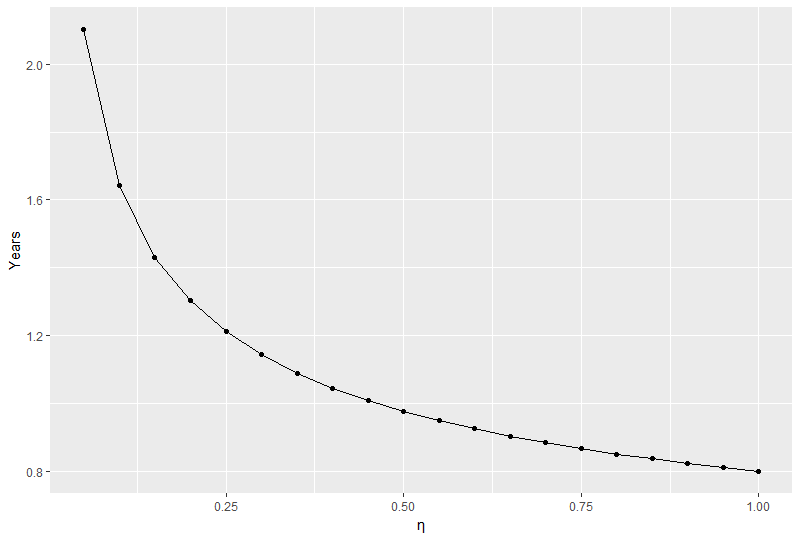
\includegraphics[width=1\textwidth]{Figures/Susceptible_Equilibrium.png}
  \caption{Time taken for susceptible intentional infection to reach the new equilibrium}
\end{figure}

\begin{figure}[H]
  \centering
  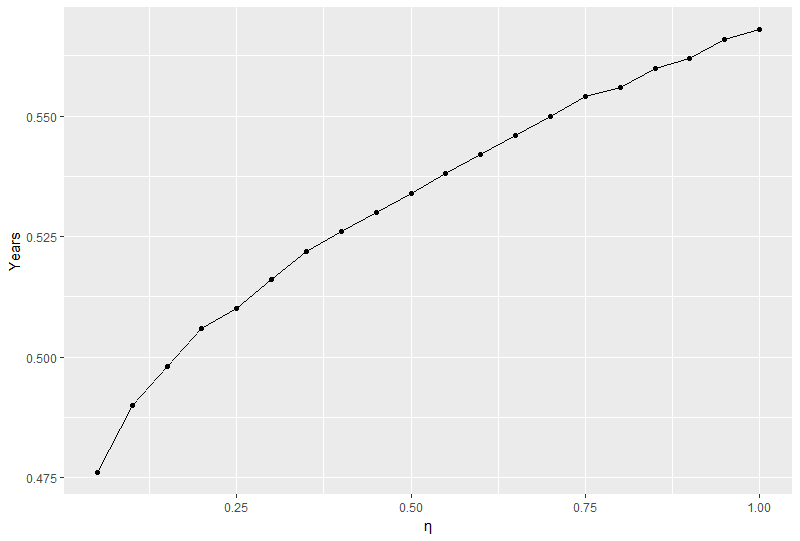
\includegraphics[width=1\textwidth]{Figures/Susceptible_advantageous.png}
  \caption{Time taken for susceptible intentional infection to have at least 10$\%$ fewer disease induced mortality, as a function of rate of intentional infection on susceptible.}
\end{figure}

Recall in \autoref{section2.2.3}, we initially found that in the newborn infection model, with a larger proportion of newborn intentional infection, it becomes more advantageous over non-intentional infection more slowly. But after we change the definition of ``more advantageous'' to be: The cumulative mortality rate of the system with intentional infection is at least 10\% less than of the system with no intentional infection, the situation was reversed. However, unlike the newborn infection model, in susceptible infection, the situation remain the same, even after the definition of ``more advantageous'' was changed. The time required for intentional infection to be more advantageous still increases as the rate of intentional infection increases. This means, with a very low rate of intentional infection on susceptible, not only can we ensure a lower cumulative mortality in the long run, but also able to be advantageous more quickly. This also means, we cannot conclude an optimal rate of intentional infection on susceptible.
\subsubsection{Comments and discussion to this model}
This model has proven the benefit of intentional infection with the approach of infecting susceptible individuals. We have shown that, with any positive rate of intentional infection on susceptible, we can always reduce the cumulative disease induced mortality, compared to not doing so. However, as we discussed in the previous section, we cannot conclude an optimal rate of intentional infection, since we have shown that the benefit is maximized, in every aspect, when the rate of intentional infection is minimal. Further study is required to answer this question.
\section{Discussion}
We have used several simple models to illustrate that both approaches of intentional infection could help restrain epidemics, by reducing the number of total death caused by life-threatening diseases, in our case, smallpox. This suggests, practices of smallpox variolation in history have indeed saved many lives. 

In addition to demonstrating the utility of intentional infection, one of our models have also shown that, under certain circumstances, the disease could be completely eradicated. Future research could perform stochastic analysis using similar systems of differential equations, in order to rigorously prove its possibility.

Even though our results have revealed that intentional infection can be an effective tool against epidemics, our mathematical models rely on several important assumptions. First, we assume that recovered individuals acquires permanent immunity against this infectious disease. Although unrealistic for many diseases, such as flu, but still applicable to many others, specifically, diseases such that infection could provide long term immunity up to several decades, for example, measles, whooping cough, etc \cite{amanna2007duration}. Secondly, in addition to our first assumption, we ignored the possibility of evolution, which is extremely common in viruses, as they mutate much faster than most of the organisms on earth \cite{purcell2000hepatitis}. Mutations may lead to different strains of viruses, so that the old immunity may not be effective anymore. Finally, we assumed a single homogeneous population, which does not account for spatial, seasonal and individual heterogeneity.

Moreover, due to the existence of special events or accidents in realistic scenarios, patterns of disease spread could be significantly altered, meaning, we have many different factor not yet being considered in our models. For both approaches, the models can still be modified and developed to higher complexity. For instance, in real life, smallpox variolation is done via skin. However, since the subject used to variolate is live smallpox virus, there could be other pathways for live smallpox virus to enter respiratory system of the variolated individual, or of the other people who has physically contacted such individual. A specific example of such pathway could be touching the area of variolation, followed by touching nose or mouth. 

In such scenario, though the variolated individual might acquire symptoms much less severe than natural infections, when virus happens to enter respiratory system, a natural infection with much more serious symptoms could still occur. Therefore, possibility still exists for a variolated individual to become gravely ill. In our construction of models, the consequence of that will be, a proportion of variolated individuals ($V$) entering naturally infected class ($I$).

It is meaningful to compare the utility of intentional infection to traditional vaccination. Unlike intentional infection, a traditional vaccine is unable to transmit from one individual to another. Therefore, intuitively, if intentional infection and traditional vaccination have the same pattern of distribution, the former could spread faster than the latter. Nevertheless, the trade-off for intentional infection is to have a proportion of people still die after being intentionally infected, whereas vaccination is assumed to provide a perfect protection against infectious disease.

We may also investigate the potential of the combination of intentional infection and traditional vaccination, which is known as transmissible vaccine. It is a vaccine that is capable of spreading from one individual to another, therefore utilizes the advantage of intentional infection, as well as providing perfect protection.

At last, we could compare the results of our models to historical data of smallpox. This may help us understand the variolation history of smallpox, which can innovate us in developing safer and more effective methods for disease prevention and control.

\printbibliography

\end{document}
